\documentclass[11pt]{article}
\usepackage[utf8]{inputenc}
\usepackage[T1]{fontenc}
\usepackage{lmodern}
\usepackage[margin=1in]{geometry}
\usepackage{amsmath,amssymb}
\usepackage{booktabs}
\usepackage{tabularx}
\usepackage{listings}
\usepackage{xcolor}
\usepackage{tikz}
\usetikzlibrary{arrows.meta,positioning,fit,calc}
\usepackage[hidelinks]{hyperref}
\usepackage{url}
\usepackage[section]{placeins}   % floats stay in their section
\emergencystretch=1.5em
\let\oldsection\section
\renewcommand{\section}{\clearpage\oldsection}   % every section starts on a new page


\lstset{basicstyle=\ttfamily\small,columns=fullflexible,keepspaces=true,frame=single,
        framerule=0.4pt,rulecolor=\color{black!30},xleftmargin=4pt,xrightmargin=4pt}

\title{Running ARM Binaries on a Quantum Processor}
\author{Sergii Salata\\ Quantag IT Solutions GmbH\\ \texttt{sergii.salata@quantag-it.com}}
\date{November 2026}

\begin{document}
\maketitle

\begin{abstract}
We show that a quantum computer can, in principle, execute unmodified ARM64 (AArch64) machine code
compiled from C, and that a stored-program von Neumann architecture can be built entirely from
quantum gates. We construct a single reversible quantum circuit, using only X, CNOT, Toffoli and
Fredkin gates, that contains program memory, a program counter, instruction fetch, a decoder for
27 classes of A64 integer instructions, a register file, condition flags, data memory with a
stack, an arithmetic and logic unit with multiplication and division, and a branch unit with
function calls. The binary is not compiled into the circuit: its instruction words are loaded
as the initial state of program-memory qubits, and the same circuit runs every program that fits
its program memory and uses the implemented subset. The machine has two deliberate restrictions:
it implements a subset of AArch64 (no floating point, SIMD, or byte and halfword memory access),
and its registers are 8 to 16 bits wide, so that it reproduces AArch64 exactly only for runs whose
values fit this width. A CPU reference checks this condition for every value of a run. All results
are obtained by exact simulation of the circuit, not on quantum hardware. C programs compiled by
clang and gcc, including programs that print their results with \texttt{printf}, produce the same
output, registers, memory and control flow as an ARM CPU in every tested run whose values fit the
register width, with the state compared after every machine cycle; runs that do not fit are detected
and reported. Two further experiments run the circuit on inputs in
superposition: a superposition of two programs, and a superposed input that takes two control-flow
paths of different length; after uncomputation both interfere as expected. The circuits need from
several hundred to more than a million qubits and up to $1.6\times10^{8}$ Toffoli gates. The
construction is not efficient and gives no computational advantage; it is a proof of principle.
Code, examples and tests: \url{https://github.com/quantag/arm-qpu}.
\end{abstract}

\section{Introduction}

Today's quantum computers are coprocessors. A classical computer holds the program, decides
which gate comes next and reads the results; the quantum processor only applies the gates
it is told to apply. The von Neumann idea of a \emph{stored-program} computer---one machine,
whose behaviour is set by a program held in its own memory and interpreted by a fetch,
decode and execute cycle---has been studied for quantum computers mostly as an architectural
or theoretical model~\cite{mariantoni2011,wang2022prototype,liu2023survey,wang2024family,yuan2024qcm,zhang2025qrm}.

In this paper we take the most literal route. We ask whether a quantum computer can run the
\emph{same machine code} as a conventional processor: the bytes that a standard C compiler
produces for an ARM64 CPU, unmodified. We answer this in the affirmative by building a
quantum circuit that interprets AArch64 instructions~\cite{armarm}. The circuit is a complete
stored-program machine: the program lives in qubits, a program counter held in qubits selects
the next instruction, a decoder made of gates determines what it means, and the execution
units update registers, flags and memory. Nothing in the circuit is measured or decided
classically while it runs.

Classical reversible computation embeds in quantum computation because the Toffoli gate is
universal for reversible logic~\cite{toffoli1980,fredkin1982,nielsen2010}. That such a machine
can exist is therefore not in doubt. What is new is a working, tested construction for a
real, widely used instruction set, driven by real compiler output, with a reference CPU
checking every run.

We are explicit about what this is not. It is not efficient: a single machine cycle costs
hundreds of thousands of gates, and a short C program needs hundreds of thousands to more
than a million qubits. It is not a speed-up: a classical program executed on a quantum
computer is simply a very expensive reversible computer. It has not been run on physical
quantum hardware, which is orders of magnitude too small and too noisy for it. The results
are obtained by exact simulation of the circuit. The contribution is a demonstration of
principle, and a verified bridge from ordinary binaries to quantum circuits.

This paper is a demonstration of principle under three explicit restrictions: a subset of the
instruction set (Section~\ref{sec:isa}), a reduced register width whose exactness is checked
(Section~\ref{sec:wbit}), and exact simulation instead of hardware (Section~\ref{sec:eval}).
Our contributions are:
\begin{itemize}
  \item a quantum stored-program machine for a substantial subset of AArch64 (27 instruction
        classes covering integer arithmetic, logic, shifts, multiply and divide, conditional
        select and compare, all common branches and calls, and 32/64-bit loads and stores with
        all addressing modes);
  \item a toolchain that loads ELF and Mach-O objects produced by clang or gcc, links them,
        runs them on the quantum machine and on a CPU reference, and reports the comparison;
  \item support for \texttt{printf}, \texttt{puts} and \texttt{putchar}, so that ordinary
        C programs print their results as if they had been run locally;
  \item an evaluation by differential testing against an ARM CPU emulator, with the machine
        state compared after every cycle, and two experiments on inputs in superposition:
        a superposition of two programs, and a superposed input that drives the machine along
        two control-flow paths of different length;
  \item a comparison of the interpreter's cost with a reversible circuit specialised for one
        function.
\end{itemize}

\section{Background and related work}

\paragraph{Quantum von Neumann architectures.}
Mariantoni et al.~\cite{mariantoni2011} demonstrated a superconducting quantum processor
exchanging data with a quantum memory; the instructions were stored on a classical computer.
Wang and coworkers developed theoretical models of a universal quantum von Neumann
architecture with quantum program memory, control unit and processing unit
\cite{wang2022prototype,liu2023survey,wang2024family}. These works treat programs as quantum
states in general; our machine stores classical programs in qubits and interprets a
classical instruction set.

\paragraph{Quantum control flow.}
Yuan, Villanyi and Carbin~\cite{yuan2024qcm} prove that a classical conditional jump cannot
be lifted to a program counter in superposition: the transition function of a jump is not
injective, so no quantum embedding exists without an auxiliary history, and that history is
entangled with the data. They give necessary and sufficient conditions (injectivity and
synchronisation) and define the Quantum Control Machine, an instruction set whose program
counter advances by a branch register. Zhang and Ying~\cite{zhang2025qrm} propose the Quantum
Register Machine, with quantum control flow (\texttt{qif}/\texttt{fiq}), recursion and a
partial-evaluation step that synchronises branches. Both define new instruction sets; our
machine executes an existing one, and Section~\ref{sec:vonneumann} relates its design to their
conditions. Yuan and Carbin also study data structures in superposition~\cite{yuan2022tower}.

\paragraph{Classical CPUs on quantum computers.}
Fitzjohn et al.\ built Qx86~\cite{fitzjohn2022,fitzjohn2024}, an Intel 8080/Z80 emulator in
which instructions are executed by quantum circuits on IBM hardware. Their program counter,
fetch and decode remain classical, and each instruction runs as a separate quantum job. In
our machine fetch, decode and control flow are themselves part of one quantum circuit.

\paragraph{Reversible computing.}
Landauer~\cite{landauer1961} and Bennett~\cite{bennett1973} showed how irreversible
computation can be embedded in reversible computation by keeping or uncomputing history.
Reversible processor architectures and instruction sets have been designed for classical
reversible hardware~\cite{axelsen2007,vieri1999}. Compilers from high-level code to reversible
circuits exist~\cite{amy2017reverc}; they compile a program into a circuit, whereas our
circuit is an interpreter that is independent of the program.

\section{The quantum stored-program machine}
\label{sec:machine}

\subsection{Machine state}

The machine is parameterised by a register width $W$ (between 8 and 16 bits), the number of
program-memory slots $S$ (a power of two), the size of data memory and the number of machine
cycles $T$. Its state consists of qubit registers:
\begin{itemize}
  \item \textbf{program memory}: $S$ words of 32 qubits, one A64 instruction word each;
  \item \textbf{program counter} (PC): $\log_2 S$ qubits, an instruction index;
  \item \textbf{register file}: the general-purpose registers X0--X30 that the program uses,
        and the stack pointer SP, $W$ qubits each;
  \item \textbf{flags}: N, Z, C, V;
  \item \textbf{data memory}: 4-byte cells of $W$ qubits;
  \item a \textbf{running} qubit, cleared when the program halts.
\end{itemize}
A program is loaded by preparing the computational basis state that holds its instruction
words in program memory, the entry point in the PC, the arguments in X0--X7 and the initial
data in data memory. The circuit itself is the same for every program that fits its program
memory and uses the implemented instruction classes.

\subsection{One machine cycle}

The circuit is $T$ repetitions of one machine cycle. Each cycle is a reversible block in five
phases (Figure~\ref{fig:cycle}):

\begin{enumerate}
  \item \textbf{Fetch.} The instruction register (32 scratch qubits) receives
        $\mathrm{IR} \mathrel{\oplus}= \mathrm{MEM}[\mathrm{PC}]$. For each slot, a comparator on
        the PC qubits computes a select qubit, and Toffoli gates copy that slot's word.
  \item \textbf{Decode.} Each instruction class is a (mask, value) pattern on the IR bits; a
        multi-controlled NOT per class, also controlled by the running qubit, yields one-hot
        class flags. If no class matches, a trap qubit is set and the machine halts.
  \item \textbf{Execute.} Register reads are multiplexers on the register fields of the IR.
        The execution units then compute, on scratch qubits: a ripple-carry adder with
        carry and overflow, a barrel shifter, a shift-and-add multiplier, a restoring
        divider, the decoder for logical bitmask immediates, condition evaluation on NZCV,
        address generation for loads and stores, and the next PC.
  \item \textbf{Copy out, then uncompute.} The cycle's results (the values to be written,
        the write enables, the new flags, the next PC, memory write data and enables) are
        copied with CNOTs into fresh per-cycle registers. The whole compute block is then
        applied in reverse, so that every scratch qubit returns to $|0\rangle$.
  \item \textbf{Commit.} Controlled-SWAP gates move the per-cycle results into the
        architectural registers, flags and memory cells. The displaced old values stay
        behind in the per-cycle registers. The next PC simply becomes the PC register of
        the following cycle; the old PC register stays behind as well.
\end{enumerate}

\begin{figure}[t]
\centering
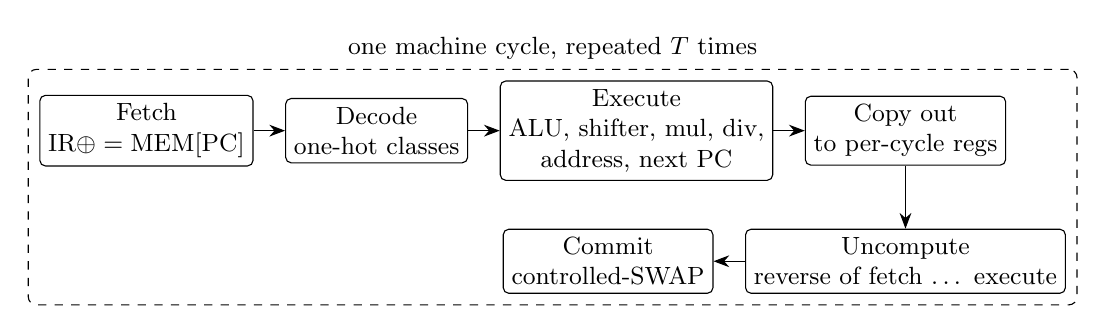
\begin{tikzpicture}[node distance=4mm, every node/.style={font=\small},
  box/.style={draw, rounded corners=2pt, minimum height=8mm, align=center, inner sep=3pt},
  arr/.style={-{Stealth[length=2mm]}}]
\node[box] (f) {Fetch\\ $\mathrm{IR}\oplus=\mathrm{MEM[PC]}$};
\node[box, right=of f] (d) {Decode\\ one-hot classes};
\node[box, right=of d] (e) {Execute\\ ALU, shifter, mul, div,\\ address, next PC};
\node[box, right=of e] (c) {Copy out\\ to per-cycle regs};
\node[box, below=8mm of c] (u) {Uncompute\\ reverse of fetch \dots\ execute};
\node[box, left=of u] (m) {Commit\\ controlled-SWAP};
\draw[arr] (f) -- (d); \draw[arr] (d) -- (e); \draw[arr] (e) -- (c);
\draw[arr] (c) -- (u); \draw[arr] (u) -- (m);
\node[draw, dashed, rounded corners=3pt, fit=(f)(d)(e)(c)(u)(m), inner sep=4pt,
      label={[font=\small]above:one machine cycle, repeated $T$ times}] {};
\end{tikzpicture}
\caption{The reversible machine cycle. Scratch qubits used in fetch, decode and execute are
returned to $|0\rangle$ by the uncompute phase; results reach the machine state only
through controlled-SWAPs in the commit phase.}
\label{fig:cycle}
\end{figure}

This is a Landauer embedding~\cite{landauer1961,bennett1973}. Overwriting a register or
jumping are not injective operations, but swapping the new value in and keeping the old one
is unitary. The price is $O(W)$ history qubits per cycle for each written register and memory
cell, plus the old PC. The PC history doubles as a complete execution trace.

\subsection{Halting and a fixed number of cycles}
\label{sec:halt}

The entry function is called with its link register (X30) pointing at a reserved program slot that
holds the instruction \texttt{HLT}. When the function returns, the machine reaches \texttt{HLT} and
clears the running qubit. Every remaining cycle is then the identity on the machine state: all class
flags are controlled by the running qubit, so nothing is written and the next PC equals the PC. The
number of cycles $T$ is fixed in advance and need only be at least the number of instructions the
program executes.

This padding makes the circuit independent of how long a particular input runs, and all inputs end
with the PC at the \texttt{HLT} slot and the running qubit cleared. It does \emph{not} make the
control state independent of the input. The per-cycle history registers still hold the PC of every
cycle and every overwritten value, and these depend on the path the run took. In the terms of
Yuan et al.~\cite{yuan2024qcm}, the machine is injective but not history-free, so the control state
at the end is not synchronised: for an input in superposition, the branches remain entangled with
their histories. Section~\ref{sec:uncompute} describes how this history is removed.

\subsection{Clearing the history by uncomputation}
\label{sec:uncompute}

Let $U$ be the whole circuit of $T$ cycles, $x$ the input (program, arguments, initial memory) and
$h(x)$ the history it leaves behind. Then
\[
  U\,|x\rangle|0\rangle_{\mathrm{hist}} = |s(x)\rangle|h(x)\rangle ,
\]
where $s(x)$ is the final machine state. Bennett's construction~\cite{bennett1973} removes the
history: copy the part of the final state that is the result, $y(x)$ (for example X0), into a fresh
register with CNOT gates, and apply $U^{-1}$:
\[
  U^{-1}\,\mathrm{COPY}_{y}\,U\;|x\rangle|0\rangle|0\rangle_{\mathrm{out}}
  = |x\rangle|0\rangle|y(x)\rangle .
\]
$U^{-1}$ is the gate list of $U$ in reverse order, because X, CNOT, Toffoli and Fredkin gates are
their own inverses. Afterwards the input, the machine state and all history registers are as they
were at the start, and only the output register depends on $x$. The control state is then the same
for every input, which is what synchronisation requires, and the circuit is a clean oracle that can
act on inputs in superposition. A phase oracle is obtained in the same way, with a phase gate on the
result in place of the copy. The cost is a factor of about two in gates and the qubits of the output.
Section~\ref{sec:branching} shows the difference experimentally: with uncomputation, two branches of
different length interfere; without it, they do not.

\subsection{The \texorpdfstring{$W$}{W}-bit model and when it is exact}
\label{sec:wbit}

AArch64 registers are 64 bits wide, which would make every adder, multiplier and divider large. Our
registers have $W$ bits, $8\le W\le16$. A $W$-bit register represents the 64-bit value (or, for
32-bit instructions, the 32-bit value) obtained by sign-extending it. We say that a value $v$ of width
$d\in\{32,64\}$ \emph{fits} if $v \equiv \mathrm{sext}_d(v \bmod 2^W)$, or if it is a pointer into the
machine's code or data memory (Section~\ref{sec:software}); pointers are represented by their offset.

The machine computes, for every instruction, the low $W$ bits of its AArch64 result from the low $W$
bits of its operands. This is exact unconditionally for operations whose low bits depend only on
the low bits of the operands, and exact under a fit condition for the others:

\begin{center}
\small
\begin{tabularx}{\textwidth}{@{}>{\raggedright\arraybackslash}p{0.47\textwidth}>{\raggedright\arraybackslash}X@{}}
\toprule
operations & condition for an exact low-$W$-bit result \\
\midrule
ADD, SUB, MUL, MADD, MSUB, AND, ORR, EOR, BIC, ORN, EON, LSL, MOVZ/MOVN/MOVK, ADRP, byte and halfword operand extensions & none; the low $W$ bits are determined by the low $W$ bits of the operands \\
LSR, ASR (immediate, register, shifted operands), UBFM/SBFM, SDIV, UDIV, SMULL, UMULL, CBZ, CBNZ, TBZ, TBNZ, CSEL family, word and doubleword extensions & the source registers fit at the width they are read \\
flag-setting forms: ADDS, SUBS, ANDS, BICS, CMP, CMN, TST, CCMP, CCMN & the operands after shift or extension, and the full-width result, fit \\
loads and stores & the stored register fits; for a 64-bit load, the doubleword in memory fits \\
\bottomrule
\end{tabularx}
\end{center}

\noindent If every instruction of a run satisfies its condition and every value written to a
register fits, then by induction over the cycles the machine state after each cycle equals the low
$W$ bits of the AArch64 state, including NZCV and the PC. The CPU reference checks these conditions
for every instruction it executes: it checks every register read at the width at which it is read
(64 bits for addresses, 32 or 64 bits for data), every register written, the second operand and the
full result of every flag-setting instruction (including those whose result is discarded, such as
\texttt{cmp}), and every memory access. A run with no violation is reported as exact. A run with a
violation is \emph{flagged}; it may still match.

The check is sound only if the circuit implements each sub-form correctly. That is tested directly:
every test compares the machine state with the CPU after every cycle (Section~\ref{sec:eval}). An
earlier version of the machine treated the byte extensions UXTB and SXTB in \texttt{add (extended
register)} as the identity, which is wrong for $W>8$ (for example, with $W=12$ and $\mathrm{X1}=256$,
\texttt{add x0, x0, w1, uxtb} gave 256 instead of 0). The defect was found in review and fixed, and the
boundary tests of Section~\ref{sec:eval} now cover every extension at every width.

A typical value that does not fit is the result of division by a constant, which compilers turn
into a multiplication by a 32-bit ``magic'' constant.

\section{How the machine realises the von Neumann architecture}
\label{sec:vonneumann}

The defining features of a von Neumann (stored-program) computer are that the program is
data held in the machine's memory, and that a fixed control unit runs a fetch, decode and
execute cycle that interprets it. Our circuit has both:

\begin{itemize}
  \item \textbf{The program is state, not structure.} The circuit contains no gate that
        depends on the program. Loading a different binary changes only the initial basis
        state of the program-memory qubits. In our tests one circuit, built once per register
        width, executes thousands of different programs.
  \item \textbf{Fetch, decode and execute are quantum operations.} The PC is a qubit
        register; the instruction is selected by gates controlled by the PC qubits; the
        decoder is a network of multi-controlled NOTs; branches compute the next PC in
        qubits. No intermediate measurement, and no classical decision, occurs inside the
        circuit.
  \item \textbf{Control flow depends on data.} Conditional branches, loops and calls,
        including returns through a register, are evaluated by the circuit from register
        and flag qubits.
\end{itemize}

Program memory and data memory are separate qubit registers, so physically the organisation
resembles a Harvard machine. Logically it is a stored-program machine: instructions are data
in qubits, and the same circuit interprets every program within its supported subset and memory size. The program memory is read-only,
which excludes self-modifying code.

Because the construction is a Landauer embedding, it respects the theorem
of~\cite{yuan2024qcm}: the history registers make the transition injective. For inputs in
the computational basis---an ordinary binary run with ordinary inputs---this is all that is
needed. For inputs in superposition the history is entangled with the data, and the
uncomputation of Section~\ref{sec:uncompute} removes it. The experiments of
Sections~\ref{sec:coherence} and~\ref{sec:branching} use this structure.

\section{Implemented instructions}
\label{sec:isa}

Table~\ref{tab:isa} lists the instructions the decoder implements, by class. The classes are
(mask, value) patterns over the instruction word, and the same table drives the quantum
decoder and the static support check of the loader, so a binary is reported as supported
exactly when the circuit can decode every instruction it contains. Both 32-bit (W register)
and 64-bit (X register) forms are implemented where they exist.

\begin{table}[t]
\centering
\small
\begin{tabularx}{\textwidth}{@{}lX@{}}
\toprule
group & instructions \\
\midrule
move & MOVZ, MOVN, MOVK and the MOV aliases \\
arithmetic & ADD, ADDS, SUB, SUBS with immediate, shifted-register and extended-register operands; CMP, CMN, NEG \\
logic & AND, ORR, EOR, ANDS, BIC, ORN, EON, BICS with register and bitmask-immediate operands; TST, MVN \\
shifts, bitfields & LSL, LSR, ASR (immediate and register); UBFM, SBFM and their aliases UBFX, SBFX, UBFIZ, SBFIZ, UXTB/H, SXTB/H/W \\
multiply, divide & MUL, MADD, MSUB, MNEG, SMULL, UMULL, SMADDL, UMADDL, SMSUBL, UMSUBL, SDIV, UDIV \\
conditional & CSEL, CSINC, CSINV, CSNEG and the aliases CSET, CSETM, CINC, CNEG; CCMP, CCMN \\
branches & B, B.cond, CBZ, CBNZ, TBZ, TBNZ, BL, BLR, BR, RET \\
memory & LDR, STR (W and X), LDRSW with unsigned offset, unscaled offset (LDUR, STUR), pre-index, post-index and register offset (LSL, UXTW, SXTW); LDP, STP with offset, pre- and post-index \\
addresses & ADRP (with ADD \texttt{:lo12:} for string literals and globals) \\
other & NOP and hints; HLT ends the run \\
\bottomrule
\end{tabularx}
\caption{AArch64 instructions implemented by the quantum decoder (27 classes).}
\label{tab:isa}
\end{table}

Not implemented are byte and halfword loads and stores, rotations (ROR, RORV), bitfield
insert (BFI, BFXIL), bit counting and reversal (CLZ, RBIT, REV), ADR, floating point, SIMD and
system instructions. A binary that contains them can still run if it never reaches them; the
report lists each one, and a run that reaches one halts with a trap. Table~\ref{tab:isa}
covers the instructions that clang and gcc emit for typical integer C code at optimisation
levels \texttt{-O0} to \texttt{-O2}: loops, arithmetic, comparisons, function calls with stack
frames, local arrays, and string literals passed to \texttt{printf}.

\subsection{Worked example: from a C expression to gates}
\label{sec:example}

We follow one line of C through the machine. Compiled with \texttt{clang -O1},
\begin{lstlisting}[language=C]
int add3(int a) { return a + 3; }
\end{lstlisting}
becomes two instructions:
\begin{lstlisting}[language={}]
0:  11000c00   add  w0, w0, #3
4:  d65f03c0   ret
\end{lstlisting}

\paragraph{The instruction word.} Table~\ref{tab:enc} shows how \texttt{0x11000c00} encodes
``add immediate'': bits 28--23 select the class, \texttt{imm12} holds the constant 3, and
\texttt{Rn} and \texttt{Rd} name register 0. In the machine these 32 bits are the basis state
of the 32 qubits of program-memory slot 0.

\begin{table}[h]
\centering
\small
\begin{tabular}{@{}lccccccc@{}}
\toprule
bits & 31 & 30 & 29 & 28--23 & 22 & 21--10 & 9--5 \,/\, 4--0 \\
field & sf & op & S & class & sh & imm12 & Rn \,/\, Rd \\
value & 0 (32-bit) & 0 (add) & 0 (no flags) & \texttt{100010} & 0 & \texttt{000000000011} = 3 & 0 \,/\, 0 \\
\bottomrule
\end{tabular}
\caption{Fields of \texttt{add w0, w0, \#3} (\texttt{0x11000c00}).}
\label{tab:enc}
\end{table}

\paragraph{Fetch.} With PC $=0$, the comparator for slot 0 sets a select qubit, and 32 Toffoli
gates controlled by it and by the slot's qubits copy the word into the instruction register
IR.

\paragraph{Decode.} The class ``add/sub immediate'' is the pattern \texttt{100010} on IR bits
28--23. Its flag is a single multi-controlled NOT with seven controls, the six IR bits
and the running qubit:
\[
  f_{\mathrm{addimm}} \mathrel{\oplus}= r \wedge \mathrm{IR}_{28} \wedge \overline{\mathrm{IR}_{27}}
  \wedge \overline{\mathrm{IR}_{26}} \wedge \overline{\mathrm{IR}_{25}} \wedge \mathrm{IR}_{24}
  \wedge \overline{\mathrm{IR}_{23}} .
\]
Negated controls are X gates before and after; the seven-control NOT is a chain of 11
Toffoli gates through 5 ancillas. Every other class has its own flag; for this word only
$f_{\mathrm{addimm}}$ becomes 1. Sub-fields are read directly from IR: $\mathrm{IR}_{30}$ (add or
subtract), $\mathrm{IR}_{29}$ (set flags), $\mathrm{IR}_{22}$ (shift of the immediate).

\paragraph{Operands.} The first operand $A$ is register Rn, read by a multiplexer: for each
register $k$, a select qubit $(\mathrm{IR}_{9..5} = k) \wedge \mathrm{enable}$ (a six-control NOT)
controls $W$ Toffoli gates that copy $X_k$ into $A$. The second operand is the immediate,
$B_i \mathrel{\oplus}= f_{\mathrm{addimm}} \wedge \overline{\mathrm{IR}_{22}} \wedge \mathrm{IR}_{10+i}$, so
$B = 3$.

\paragraph{Addition.} The adder works out of place. With $p = A$, $q = B$ (inverted for
subtraction) and $c_0$ the carry-in, every bit $i$ produces a fresh sum qubit and a fresh
carry qubit,
\[
  s_i = p_i \oplus q_i \oplus c_i, \qquad
  c_{i+1} = \mathrm{maj}(p_i, q_i, c_i) = p_i q_i \oplus p_i c_i \oplus q_i c_i ,
\]
which is three CNOT and three Toffoli gates (Figure~\ref{fig:slice}). For $W = 8$ the adder is
24 CNOT and 24 Toffoli gates. The carries also give the C and V flags.

\begin{figure}[h]
\centering
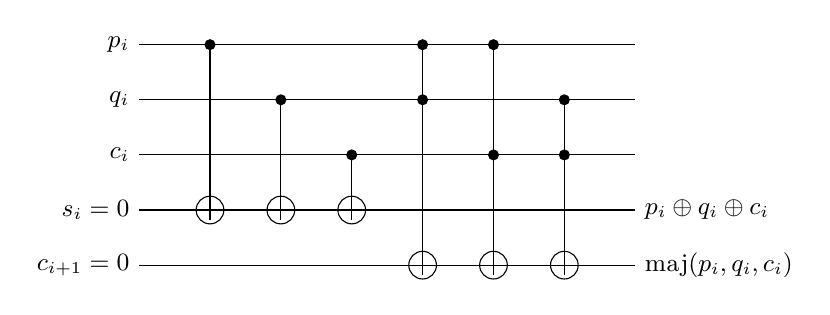
\begin{tikzpicture}[x=9mm, y=7mm, every node/.style={font=\small}]
  \foreach \y/\l in {4/{p_i}, 3/{q_i}, 2/{c_i}, 1/{s_i = 0}, 0/{c_{i+1} = 0}}
    { \node[left] at (0,\y) {$\l$}; \draw (0,\y) -- (7,\y); }
  \node[right] at (7,1) {$p_i \oplus q_i \oplus c_i$};
  \node[right] at (7,0) {$\mathrm{maj}(p_i, q_i, c_i)$};
  % CNOTs onto s_i
  \foreach \x/\c in {1/4, 2/3, 3/2} {
    \fill (\x,\c) circle (2pt); \draw (\x,\c) -- (\x,1);
    \draw (\x,1) circle (5pt); \draw (\x,1-0.18) -- (\x,1+0.18); }
  % Toffolis onto c_{i+1}
  \foreach \x/\a/\b in {4/4/3, 5/4/2, 6/3/2} {
    \fill (\x,\a) circle (2pt); \fill (\x,\b) circle (2pt); \draw (\x,\a) -- (\x,0);
    \draw (\x,0) circle (5pt); \draw (\x,-0.18) -- (\x,0.18); }
\end{tikzpicture}
\caption{One bit of the adder: three CNOTs compute the sum bit and three Toffoli gates
compute the carry (majority) into fresh qubits.}
\label{fig:slice}
\end{figure}

\paragraph{Result and write-back.} The result register receives $R_i \mathrel{\oplus}=
f_{\mathrm{addimm}} \wedge s_i$. The write enable of register $k$ is
$(\mathrm{IR}_{4..0} = k) \wedge \mathrm{writes}$. $R$ and the enables are copied with CNOTs into
fresh per-cycle qubits, the compute block runs backwards so that IR, flags, $A$, $B$, the
sums and the carries return to $|0\rangle$, and the commit phase applies
$\mathrm{CSWAP}(\mathit{we}_0, X_{0,i}, R'_i)$ for $i < W$. Afterwards X0 holds $a + 3$ and
$R'$ holds the old value of X0. The next PC, $\mathrm{PC} + 1$, comes from the same adder
structure on the PC qubits, and the following cycle fetches \texttt{ret}.

\paragraph{Cost.} On a machine whose decoder implements only the classes this function needs
(add/sub immediate, register branches and \texttt{HLT}), with $W = 8$, two registers and four
program slots, one complete cycle is 1\,590 gates: 1\,034 Toffoli, 134 CNOT, 394 X and 28
Fredkin gates, on 321 qubits. The full machine with all 27 classes and realistic memory sizes
uses about $4\times10^{5}$ gates per cycle. The arithmetic itself is a small part of this;
most of the cost is in the multiplexers over program memory, data memory and registers, and
in the units that every cycle computes, such as the divider, whether the current instruction
needs them or not.

\section{Software structure}
\label{sec:software}

The implementation is a Python program, \texttt{arm\_qpu.py}, and a package \texttt{qcpu}
\cite{armqpu}. Figure~\ref{fig:pipeline} shows the flow from a C source file to a result.

\begin{figure}[t]
\centering
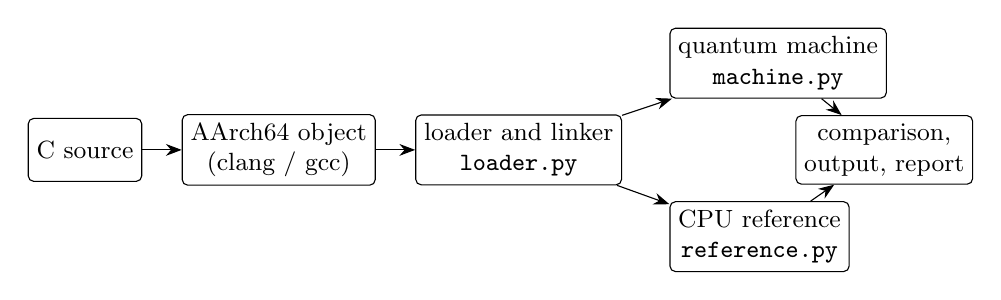
\begin{tikzpicture}[node distance=5mm, every node/.style={font=\small},
  box/.style={draw, rounded corners=2pt, minimum height=8mm, align=center, inner sep=3pt},
  arr/.style={-{Stealth[length=2mm]}}]
\node[box] (c) {C source};
\node[box, right=of c] (o) {AArch64 object\\ (clang / gcc)};
\node[box, right=of o] (l) {loader and linker\\ \texttt{loader.py}};
\node[box, above right=2mm and 6mm of l] (q) {quantum machine\\ \texttt{machine.py}};
\node[box, below right=2mm and 6mm of l] (r) {CPU reference\\ \texttt{reference.py}};
\node[box, right=22mm of l] (cmp) {comparison,\\ output, report};
\draw[arr] (c) -- (o); \draw[arr] (o) -- (l);
\draw[arr] (l) -- (q); \draw[arr] (l) -- (r);
\draw[arr] (q) -- (cmp); \draw[arr] (r) -- (cmp);
\end{tikzpicture}
\caption{From C source to a checked quantum run.}
\label{fig:pipeline}
\end{figure}

\paragraph{Compilation.} The user compiles C with clang or gcc for AArch64 into an object
file, for example \texttt{clang --target=aarch64-linux-gnu -O1 -c prog.c}. Both compilers,
ELF objects, and arm64 Mach-O objects from Apple's toolchain are supported.

\paragraph{Loader and linker} (\texttt{qcpu/loader.py}). The loader merges all executable
sections into one code image and places the data sections (\texttt{.rodata}, \texttt{.data},
\texttt{.bss}, string literals) in data memory. It applies the relocations a linker would:
branches and calls (CALL26, JUMP26, BRANCH26), page addresses (ADR\_PREL\_PG\_HI21, PAGE21),
page offsets (ADD\_ABS\_LO12\_NC, LDST$n$\_ABS\_LO12\_NC, PAGEOFF12) and absolute pointers in
data (ABS64). Calls to \texttt{printf}, \texttt{puts} and \texttt{putchar} are bound to an
output stub (Section~\ref{sec:printf}). The last program slot receives the \texttt{HLT}
instruction, and the memory layout places the output log, the data sections, user data and
the stack.

\paragraph{Static check} (\texttt{qcpu/a64.py}). Every instruction word is classified by the
same class table as the quantum decoder, with additional checks for unallocated and
unimplemented sub-forms.

\paragraph{Quantum machine} (\texttt{qcpu/machine.py}). The circuit generator emits the gate
list of Section~\ref{sec:machine}. It decomposes multi-controlled NOTs into Toffoli chains with
ancillas from a pool that is reused in every cycle, and it builds each functional unit out of
place so that it can be uncomputed. The circuit can be exported to Qiskit~\cite{qiskit2024}.

\paragraph{CPU reference and model check} (\texttt{qcpu/reference.py}). The same bytes run on
the Unicorn emulator~\cite{unicorn}, which uses QEMU's ARM CPU core, one instruction at a
time and with the same memory layout. The reference records the PC trace and checks every
value against the $W$-bit model of Section~\ref{sec:wbit}, including flag-setting results
that are discarded and every memory access.

\paragraph{Simulation and backends} (\texttt{qcpu/bitsim.py}). Because the circuit uses only
X, CNOT, Toffoli and Fredkin gates, it maps computational basis states to computational basis
states, and a basis-state input can be simulated exactly by tracking bits. Every cycle is the
same gate list; only its per-cycle registers are new qubits. The simulator therefore
generates one cycle once and replays it $T$ times, resetting the per-cycle qubits and feeding
in the previous cycle's PC, which is the same computation as the full circuit without
storing $10^8$ gates. For inputs in superposition the circuit is run on Qiskit Aer, and an
IBM Quantum backend is provided that checks the circuit's width against the device before
submitting.

\paragraph{Runner} (\texttt{arm\_qpu.py}). By default the runner prints only the program's
own output and returns \texttt{main}'s return value as its exit code, as if the binary had
been run locally. With \texttt{-v} it also prints the comparison with the CPU and the
circuit's resources, and writes a report with the annotated disassembly, the instructions
executed, the comparison of registers, flags, memory and PC trace, and the model check.

\section{Program output: \texttt{printf}}
\label{sec:printf}

Printing is input/output, not computation, and on a quantum computer it raises a specific
question: how can text leave a circuit that must stay coherent until the end? A system call
that interrupts the circuit to print would require a measurement in the middle of the run.
We instead treat output the way a hardware device does.

\paragraph{Output stub.} The linker binds \texttt{printf}, \texttt{puts} and \texttt{putchar}
to a stub of 33 A64 instructions, which is listed in the repository
(\texttt{docs/output\_stub.s}). The stub runs on the quantum machine like any other code. Each
call appends one 32-byte record to an \emph{output log} at the start of data memory: the kind
of call, the address of the format string, and the first six integer or pointer arguments.
A counter at the start of the log is incremented, and calls beyond the log's capacity are
dropped. On Apple's arm64 ABI, variadic arguments are passed on the stack; a variant of the
stub loads them from there.

\paragraph{Formatting on the host.} After the run, the output log is read from the final data
memory, which is measured together with the rest of the machine state, and formatted on the
host with the rules of C's \texttt{printf}. Format strings and \texttt{\%s} arguments are read
from the program's constant data (\texttt{.rodata}). The CPU reference executes the same stub,
so the host renders both machines' output and compares them.

\paragraph{What runs where.} All computation runs on the quantum machine, including every value
that is printed, the decision of what to print and when, and the order of the calls. Only the
conversion of the logged values into characters happens classically, after the final
measurement. The program is unaware of this: it includes \texttt{<stdio.h>} (a minimal header
is provided, so no system headers or C library are needed) and calls \texttt{printf} as usual.
Compilers turn \texttt{printf("text\textbackslash n")} into \texttt{puts}, which is why the
stub also covers \texttt{puts} and \texttt{putchar}.

\paragraph{Return values.} \texttt{putchar(c)} returns \texttt{c} and \texttt{puts} returns 0, as C
requires (a non-negative value on success). \texttt{printf} returns 0 instead of the number of characters
written: that number is only known when the text is formatted, after the run. Programs that use the
return value of \texttt{printf} are therefore not supported.

\paragraph{Limits.} Integers and pointers are supported, floating point is not; up to six
arguments per call; \texttt{\%s} works for constant strings, not for text built in memory at run
time (byte loads are not implemented); and the log holds a configurable number of calls
(32 by default).

Listing~\ref{lst:hello} shows a complete program, and how it is compiled and run.

\begin{lstlisting}[language=C,caption={A C program and its run on the quantum machine.},label={lst:hello}]
#include <stdio.h>

int smallest_factor(int n) {
    for (int d = 2; d * d <= n; d++)
        if (n % d == 0) return d;
    return n;
}

int main(void) {
    int n = 84;
    printf("Hello from the QPU!\n");
    printf("%d =", n);
    while (n > 1) {
        int p = smallest_factor(n);
        printf(" %d", p);
        n /= p;
    }
    printf("\n");
    return 0;
}
\end{lstlisting}
\begin{lstlisting}[language={}]
$ clang --target=aarch64-linux-gnu -O1 -fno-stack-protector \
        -Iinclude -c hello.c -o hello.o
$ python3 arm_qpu.py hello.o
Hello from the QPU!
84 = 2 2 3 7
\end{lstlisting}

\section{Evaluation}
\label{sec:eval}

All results in this section are obtained by exact simulation of the circuit on a classical
computer. The numbers are those of \texttt{docs/test\_results.md} in the repository, generated by
\texttt{tools/test\_report.py} from commit \texttt{5d3eeee} with Python 3.13, Qiskit 2.6.2,
Qiskit Aer 0.18.4, Unicorn 2.1.4, LIEF 1.0.0, clang 18.1.3 and aarch64-linux-gnu-gcc 13.3.0.

\subsection{Method: lockstep comparison and outcome classes}

Every run is executed twice: on the quantum machine and on the CPU reference (Unicorn). The two
are compared after \emph{every} machine cycle, not only at the end: the PC, the NZCV flags, the
low $W$ bits of every instantiated register and of every data-memory cell, and the running and
trap qubits. For programs that print, the rendered output text is compared as well. Independently,
the reference checks the conditions of Section~\ref{sec:wbit} for every instruction. Each run falls
into one of five classes:

\begin{description}
  \item[match] the states agree after every cycle and the model check is clean;
  \item[match-flagged] the states agree, but the model check reported a value outside the $W$-bit model;
  \item[flagged] the states differ, and the model check reported it;
  \item[unflagged] the states differ and the model check is silent. This is a defect of the circuit
        or of the check and must never occur;
  \item[discarded] the program was rejected by the assembler, was too long for the program memory,
        or did not halt normally on the CPU.
\end{description}

\noindent A run counts as a successful execution of ARM code only in the class \emph{match}.
The class \emph{flagged} is the expected behaviour of a reduced-width machine on values that do not
fit; what the method guarantees is that such runs are never reported as exact.

\subsection{Differential fuzzing}

A fuzzer generates random A64 programs of 4 to 13 instructions from 24 kinds of instruction,
covering all implemented classes, including every operand extension, 32- and 64-bit forms,
\texttt{smull}/\texttt{umull}, loads and stores of all addressing modes, forward branches and calls.
Register values and memory contents are random. The programs run on one interpreter circuit per
width (8 registers, 32 program slots, 32 cycles, 8 memory cells). Table~\ref{tab:fuzz} gives the
outcome of 300 programs per width, with the seeds used.

\begin{table}[htbp]
\centering
\small
\begin{tabular}{@{}rrrrrrrr@{}}
\toprule
$W$ & seed & generated & discarded & match & match-flagged & flagged & unflagged \\
\midrule
8  & 15 & 300 & 36 & 91  & 127 & 46 & 0 \\
12 & 19 & 300 & 37 & 150 & 77  & 36 & 0 \\
16 & 23 & 300 & 35 & 162 & 71  & 32 & 0 \\
\bottomrule
\end{tabular}
\caption{Differential fuzzing. All discarded programs were rejected by the assembler (random
operand combinations that A64 does not encode); none was too long or failed to halt.}
\label{tab:fuzz}
\end{table}

\subsection{Boundary cases}

A second suite runs short instruction sequences on operands at the boundaries of each width:
$0, \pm1, 2, 7, 127, 128, 255, 256, -128, -129, 0x1F0$, $2^{W-2}$, $2^{W-1}-1$, $-2^{W-1}$ and the
values $2^{W-1}$ and $-2^{W-1}-1$ just outside the model. It covers the extensions UXTB, UXTH, UXTW,
SXTB, SXTH and SXTW with shifts 0, 2 and 4 in \texttt{add} and \texttt{subs}, with W and X destinations;
\texttt{cmp} and \texttt{adds} in W and X forms followed by \texttt{cset} on all 14 conditions;
LSL, LSR and ASR by immediate (including $W-1$, $W$, 31 and 63) and by register (including 32, 64 and
$-1$), and as shifted operands; W results used as X values; loads and stores of W and X registers,
\texttt{ldrsw}, pairs with pre- and post-index writeback, and mixed 32/64-bit accesses to the same
cells; \texttt{mul}, \texttt{madd}, \texttt{smull}, \texttt{umull}, signed and unsigned division
including division by zero and $-2^{W-1}/-1$; and bitfield moves. In total 4\,730 cases ran at $W=8,12,16$
(1\,313, 1\,717 and 1\,700). Every one of them is in the classes match, match-flagged or flagged;
none is unflagged. The case of the defect reported in Section~\ref{sec:wbit} is among them.

\subsection{Fast simulator against the full circuit}

Most runs use a fast simulator: it builds the gate list of one machine cycle once and replays it
$T$ times, resetting the per-cycle qubits and feeding the PC and running qubit to the next cycle.
To check that this is the same as simulating the full circuit, 100 random programs (seed 5) were
run on both the fully materialised circuit (5\,691 qubits, 644\,920 gates) and the replay: all 100
final states are identical bit for bit, and the reported resource counts agree. Three short
programs were also run through Qiskit Aer, on the circuit exported to Qiskit (1\,101 qubits), with
the same results as the fast simulator.

\subsection{C programs}

The test suite compiles C programs with clang and with gcc at \texttt{-O0}, \texttt{-O1} and
\texttt{-O2}. It runs 16 function-level cases (trial-division factorization, gcd, Fibonacci,
primality, popcount, Collatz steps, integer square root, modular exponentiation, maximum of
three, function calls, bubble sort in memory, binary search, digit sum) and three whole
programs whose \texttt{main} prints its results with \texttt{printf}. All 54 runs per compiler
pass. 52 (clang) and 51 (gcc) of them match the CPU exactly. The remaining runs are the digit-sum
function, in which the compiler replaces division by 10 with a multiplication by a 32-bit constant
(clang at \texttt{-O1} and \texttt{-O2}, gcc at every level); the model check flags them, as
required, because their intermediate values do not fit.

Table~\ref{tab:res} lists the resources of the example programs, compiled with clang
\texttt{-O1}. The qubit and gate counts are those of the full circuit; ``cycles'' is the number
of machine cycles $T$.

\begin{table}[htbp]
\centering
\small
\begin{tabular}{@{}lrrrrrr@{}}
\toprule
program & instructions & cycles & $W$ & qubits & gates & Toffoli \\
\midrule
coherence test (Sec.~\ref{sec:coherence}) & 3 & 4 & 8 & 418 & 7\,448 & 4\,880 \\
branching test (Sec.~\ref{sec:branching}) & 6 & 13 & 8 & 868 & 42\,198 & 27\,612 \\
\texttt{factorize(84)}, one function & 230 & 72 & 12 & 179\,692 & $3.06\times10^{7}$ & $1.95\times10^{7}$ \\
\texttt{hello.c} (Listing~\ref{lst:hello}) & 87 & 228 & 12 & 520\,364 & $9.19\times10^{7}$ & $5.78\times10^{7}$ \\
\texttt{algorithms.c}, 7 results & 339 & 497 & 12 & 1\,127\,989 & $2.32\times10^{8}$ & $1.51\times10^{8}$ \\
\texttt{factor.c}, 3 factorizations & 230 & 606 & 12 & 1\,367\,842 & $2.58\times10^{8}$ & $1.64\times10^{8}$ \\
\bottomrule
\end{tabular}
\caption{Resources of the example programs (clang \texttt{-O1}). ``Instructions'' counts the
linked code image, including the output stub; the coherence and branching tests run on machines
whose decoder implements only the classes their programs use.}
\label{tab:res}
\end{table}

A full machine cycle with all 27 instruction classes, 64 to 512 program slots and data memory
costs roughly $4\times10^{5}$ gates. Its largest parts are the program-memory and data-memory
multiplexers, whose cost grows linearly with the memory sizes, and the divider. The exact
simulation of the largest example takes about 20 seconds on one CPU core.

\subsection{Coherence: a superposition of two programs}
\label{sec:coherence}

The previous results use basis-state inputs, for which a reversible classical simulation
gives the same outcome. To show that the circuit is a coherent quantum computation, we
run the program \texttt{movz w0,\#5; add w0,w0,\#3; ret} on Qiskit Aer with the
matrix-product-state method. Bit 5 of the first instruction word is bit 0 of the immediate,
so flipping it turns \texttt{\#5} into \texttt{\#4}. We apply a Hadamard gate to that
program-memory qubit before the machine runs.

\begin{enumerate}
  \item \textbf{Superposed program.} Measuring X0 after the run gives 8 or 7, with frequencies
        1017 and 983 out of 2000 shots: one run executed both programs.
  \item \textbf{Interference.} We apply $H$ to the qubit, the machine $U$, a phase $Z$ on bit 0
        of X0, the inverse machine $U^{-1}$ and $H$ again, then measure the qubit. Without the
        phase the outcome is 1 in all 2000 shots; with the phase it is 0 in all 2000 shots.
\end{enumerate}

The deterministic, flipped outcome in the second experiment requires the two program branches to
interfere. That is only possible if fetch, decode and execution are coherent: a measurement or a
classically controlled step anywhere inside $U$ would destroy the interference and give 50/50
outcomes. In this experiment both branches follow the same control-flow path; the next experiment
removes that restriction.

\subsection{Quantum branching: two paths of different length}
\label{sec:branching}

The program
\begin{lstlisting}[language={}]
f:  cbz  w0, 1f        // x = 0: return at once
    mov  w1, #3        // x = 1: loop three times
2:  add  w2, w2, #2
    subs w1, w1, #1
    b.ne 2b
1:  ret
\end{lstlisting}
is run with bit 0 of X0 in the state $(|0\rangle+|1\rangle)/\sqrt2$. For $x=0$ the machine takes the
branch and halts after 3 cycles; for $x=1$ it runs the loop and halts after 13 cycles. The branches
therefore differ in the sequence of PCs, in their length, and in their history registers. The
circuit runs 13 cycles (868 qubits, 42\,198 gates, Qiskit Aer, 2000 shots each).

\begin{enumerate}
  \item[A.] \textbf{Superposed control flow.} Measuring $x$, X2 and the running qubit of cycle 3
        gives only $(x,\mathrm{X2},\mathrm{running})=(0,0,0)$ (996 shots) and $(1,6,1)$ (1004 shots):
        after three cycles the $x=0$ branch has halted while the $x=1$ branch is still in the loop,
        and each branch ends with its own result.
  \item[B.] \textbf{Interference after uncomputation.} $H$, $U$, a phase $Z$ on bit 1 of X2, $U^{-1}$,
        $H$, measure $x$. Without the phase the outcome is 0 in all 2000 shots; with the phase it is
        1 in all 2000 shots. The phase sits on a value that only the $x=1$ branch computes, and the two
        branches, of different path and length, interfere completely.
  \item[C.] \textbf{No interference without uncomputation.} The same circuit without $U^{-1}$ gives
        988 and 1012 shots: no interference. The equal final PC and running qubit of the two branches
        (Section~\ref{sec:halt}) are not enough; their histories differ and keep them entangled with
        the data.
\end{enumerate}

Experiments B and C are the two sides of Section~\ref{sec:uncompute}: the padded machine alone is
not synchronised, and Bennett's uncomputation makes it so.

\subsection{Interpreter against a specialised reversible circuit}

To measure the price of interpretation, we compare the machine with a reversible circuit written by
hand for one function, $f(a,b)=(a+b)\cdot(a\oplus b)$ with $W=8$. Compiled, $f$ is 4 instructions
and runs in 5 machine cycles. The specialised circuit is an adder, a bitwise XOR and a multiplier on
fixed registers, with Bennett cleanup of its temporaries. It was checked on 2000 random inputs,
on which it computes $f$ and returns all temporaries to $|0\rangle$.

\begin{table}[htbp]
\centering
\small
\begin{tabular}{@{}lrrr@{}}
\toprule
circuit & qubits & gates & Toffoli \\
\midrule
interpreter, full decoder (27 classes) & 2\,012 & 110\,375 & 47\,610 \\
interpreter, decoder reduced to the classes used & 1\,047 & 30\,895 & 18\,090 \\
specialised reversible circuit & 290 & 722 & 340 \\
\bottomrule
\end{tabular}
\caption{Cost of interpretation for $f(a,b)=(a+b)\cdot(a\oplus b)$, $W=8$.}
\label{tab:spec}
\end{table}

\noindent The interpreter costs 153 times the gates and 7 times the qubits of the specialised
circuit (Table~\ref{tab:spec}). The overhead comes from fetch, decode, the multiplexers over
registers and memory, the units an instruction does not use, and the per-cycle history. Removing it
is exactly what partial evaluation of the interpreter would do (Section~\ref{sec:discussion}).

\subsection{Reproducibility}

All runs are deterministic given the seeds above. \texttt{python3 tools/test\_report.py} reruns
every experiment of this section (about 25 minutes on one core) and rewrites
\texttt{docs/test\_results.md} with the commit, the tool versions, the seeds and the number of runs in
every class, including discarded ones.

\section{Discussion}
\label{sec:discussion}

\paragraph{Cost.} The machine is extremely expensive. Each cycle re-reads the entire program
memory and data memory through multiplexers, keeps $O(W)$ history qubits per write, and
contains a multiplier and a divider even when the instruction is a move. A short C program
needs hundreds of thousands to more than a million qubits and up to $1.6\times10^{8}$ Toffoli
gates. Current devices offer on the order of a hundred to a few thousand noisy physical
qubits, so a hardware run of anything but a few-instruction program on a heavily reduced
machine profile is out of reach until large fault-tolerant machines exist.

\paragraph{No advantage.} A classical program executed this way gains nothing from being on a
quantum computer: on basis-state inputs it computes exactly what a CPU computes, many orders
of magnitude more slowly. The interest of the construction lies elsewhere. It shows concretely
that the stored-program model and real machine code can be carried by a quantum computer, it
provides a test bed for quantum control flow on a real instruction set, and, combined with
Bennett's method, it turns ordinary compiled code into reversible oracles whose correctness is
checked against a real CPU. Such oracles are needed by quantum algorithms that evaluate a
classical function in superposition, and by resource estimates for them~\cite{grassl2016aes,amy2016sha}.

\paragraph{Towards efficiency.} The interpreter can be specialised to a fixed program by
partial evaluation~\cite{futamura1971}, which removes fetch and decode and leaves a compiled
reversible circuit for that program. The history-free control flow of~\cite{yuan2024qcm} and
the synchronisation of~\cite{zhang2025qrm} point to how branching on quantum data could be
added to the instruction set. A hybrid design that keeps the PC classical wherever control
depends only on classical data would reduce the cost by orders of magnitude.

\paragraph{Limitations.} The register width $W\le16$ limits values to small integers, and runs whose
values do not fit are flagged rather than executed exactly; the instruction subset excludes byte and
halfword memory access, floating point and SIMD; program memory is read-only; output is limited to
\texttt{printf}-style records formatted after the run, and \texttt{printf} returns 0; and all results
are from simulation, not from quantum hardware.

\section{Conclusion}

We built a quantum circuit that is a stored-program computer for a subset of AArch64 with 8- to
16-bit registers, and showed in exact simulation that it runs C programs compiled by clang and
gcc---loops, function calls, arrays and \texttt{printf}---with the same state as an ARM CPU after every
cycle, whenever the run's values fit the register width; runs that do not fit are detected and
flagged. On inputs in superposition the machine executes two programs, or two control-flow paths of
different length, coherently, and after uncomputation the branches interfere. The construction is
inefficient and gives no speed-up, but it demonstrates that a quantum computer can run ARM code and
implement the von Neumann architecture. All code, examples and tests are available at
\url{https://github.com/quantag/arm-qpu}~\cite{armqpu}.

\bibliographystyle{unsrt}
\bibliography{references}

\end{document}
